%!TEX root = ../thesis.tex
\chapter{Introduction}

% We are all natural performers. Humans are proficient at demonstrating how to perform a task in action. However, articulating knowledge into a written or structured form can be extremely difficult. From dancing, repairing a machine, to operating software applications, it remains a challenge how everyday activities can be efficiently captured for a remote learner to understand.

% My research in Human-Computer Interaction supports authors in expressing their knowledge or experiences from demonstration. I develop authoring tools that dramatically increase the quality of amateur-produced content. In turn, the results engage viewers in learning.
% %
% My computational approaches enhance authoring processes from recording, editing, to replaying content.
% %
% These methods include: 1) designing novel interactive tutorials, 2) generating instructions from demonstration, and 3) storytelling from conversation.

When attempting to accomplish unfamiliar, complicated tasks, people often search for online tutorials to follow instructions. The availability of content sharing sites such as YouTube\footnote{https://www.youtube.com/} and Instructables\footnote{http://www.instructables.com/} has enabled experts and hobbyists to create tutorials for a wide spectrum of topics \cite{Lafreniere:2012tl}. From using software applications, performing physical tasks such as cooking and assembling a machine, to free-form activities like sports and dance performance, each domain involves specific ``how-to'' knowledge with a certain degree of complexity \cite{ryle1945knowhow}. Instructions, which contain the know-how and can be presented in different formats, enable novices to learn the domain knowledge and execute in action.

Among all the online support, videos are commonly used to present instructions. We suspect that users prefer videos over other formats for the following reasons:
%
First, consumer devices and software have become affordable for people to quickly record activities and later share via online platforms at minimum cost.
%
% ** describe the difficulties of making knowledge "explicit", esp. for actions and motions
Second, videos can be an efficient medium to document activities. Transferring know-how concisely and effectively to the audience is challenging. It especially requires efforts when a task involves \emph{tacit knowledge}, which is a kind of knowledge that is difficult to articulate in a written or verbal form \cite{polanyi1958personal, Klemmer:2006:BMF:1142405.1142429}. Examples of tacit knowledge include dancing, riding a bike, or driving nails with a hammer. Dancers can perform movements fluently with music. If they are asked to focus on the composite pieces, such as the arm and foot actions or rhythm, they might get confused and fail to express the entire movement. Very often, recording a video eases the difficulties of describing the entire activities in an explicit form.
%
This leads to another motivation that videos also provide an effective channel to convey ideas with adequate amounts of details. Learners can visually observe the exact actions in a video as if an expert were coaching in person.

However, while videos are easy to produce, they can include a lot of unnecessary footage. Inevitable content such as pauses, mistakes, and long repetitive actions makes it difficult for learners to focus on the most important steps and actions. Producing high-quality instructions that are easy to follow requires authoring expertise and a significant time investment in video editing practices \cite{Muller:2009tw}. A lot of effort goes into removing unnecessary footage, applying visual effects, and adding subtitles and annotations. On the other hand, given a well-edited video, navigating using a conventional video player remains inefficient. Learners with various needs could have a hard time skimming to an interesting moment or perceiving high-level overviews. Therefore, some prefer to follow static step-by-step tutorials, which are easy to scan forward and backward as instructions are listed in text and images. Similarly, it is time- and labor-intensive to produce this type of instructions.

\begin{figure}[t]
  \centering
  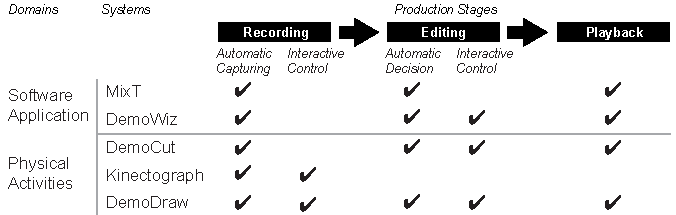
\includegraphics[width=1.0\columnwidth]{fig/space}
  \caption{A design space of the creation and consumption process for tutorials. It involves three phases of recording, editing, and playback in either software domain or a physical world. This thesis proposes a series of systems that focus on various aspects in this design space.}
  \label{fig:space}
\end{figure}

We aim to combine the advantage of ubiquitous video recording with the benefits of video and structured tutorial formats. In this thesis, we propose video-based recording, editing, and playback tools that are optimized for creating and consuming instructional demonstrations. Our goal is to dramatically increase the quality of amateur-produced video instructions, which in turn improves learning for viewers who interactively navigate the content. To support this vision, we design and develop a set of systems that encode the current practices from professional authors into automatic algorithms and interactive techniques to support amateur users. These systems cover both software applications (e.g., image manipulation tasks or browser navigation) and physical activities (e.g., Do-It-Yourself projects or dance movements), supporting different phases of the tutorial creation and consumption process (see Figure~\ref{fig:space}). Our video-based approaches consider key events or moments that are important to a learner. This information can be derived from software event logs or human annotation of physical tasks when automatic recognition remains challenging. Based on the metadata and video streams, we propose automatic methods to generate concise instructions:

\begin{itemize}
\setlength{\itemsep}{0pt}
\item \emph{MixT} captures screencast video and operation events of a software demonstration. It automatically generates mixed-media tutorials that include both static and video instructions. Learners can quickly scan through the document using text and screenshots, and follow a video clip for a certain step to observe the instructor's demo.
\item \emph{DemoWiz} is a video presentation system that provides an increased awareness of upcoming actions through glanceable visualizations. By logging the input events of a software demonstration, it overlays visual cues on the video recording to support better control of timing when re-performing a demo. Playback speed of recorded actions can be adjusted or skipped based on live presentation needs.
\item \emph{DemoCut} segments a video recording of a physical demonstration (e.g., a long cooking process) based on user annotations and video and audio analysis. It automatically applies video editing effects (e.g., skip, speedup, and zoom) to create concise instructions. A playback interface enables lightweight editing for authors to review the results.
\item \emph{Kinectograph} is a recording device that automatically tracks and follows specific body parts, e.g., hands, of an instructor in a video. It utilizes a Kinect depth sensor to track skeletal data and adjusts the camera angle via a 2D pan-tilt gimbal mount. Authors can freely move around in space to demonstrate a task and monitor real-time video preview through a tablet application.
\item \emph{DemoDraw} automatically generates motion illustrations from a RGB-D video input of a user's physical movements. It captures motions of an actor in a 3D space and enables flexible exploration of possible illustrations using different motion visualization techniques.
\end{itemize}

% \section{Challenges of Authoring and Consuming Tutorials}
\section{Thesis Contributions}

We introduce the rationale and technical challenges of these interactive system designs. Each system is evaluated both quantitatively and qualitatively to study the usability in authoring and learning. The contributions of our research include:

\begin{itemize}
  \setlength{\itemsep}{0pt}
\item New instructional formats that consider the learning factors from several domains, including software applications and physical activities.
\item Lightweight workflows in an easy-to-setup environment for amateur users to create effective instructions by demonstration.
\item Automatic or semi-automatic approaches using video and audio analysis that includes users in the loop to produce high-quality results.
\end{itemize}

\section{Overview}

The rest of my thesis is structured as follows:
%
In Chapter 2, I survey the literature on instruction consumption and creation. I review studies on why people rely on tutorials in general, how the formats of instructions matter, and the current practices of authoring instructions in several domains.

I presented two systems that support consuming tutorials for software applications.
% MixT
In Chapter 3, I present my study on how a new tutorial format supports learners in following step-by-step instructions with mixed media, including static text, images, and video clips. I introduce my creation tool called MixT, that automatically generates such new tutorial format from an author demonstration in a software application.
%
% DemoWiz
Chapter 4 introduces my authoring tool called DemoWiz, which assists consumers in capturing the timing of input events in a screencast demo video.

Then, I introduced three systems designed for real-world tasks that involve physical demonstrations.
% DemoCut
In Chapter 5,

% Kinectograph
In Chapter 6,

% DemoDraw
Finally, in Chapter 7

% Conclusion
Throughout this thesis, I ... Chapter 8 concludes my approaches for tutorials in both software and physical instructions and suggests new directions for future research on interactive tutorials.

\section {Statement on Multiple Authorship and Prior Publications}

This dissertation is based on papers published in previous ACM conference proceedings: the MixT system was published at UIST 2012 \cite{Chi:2012fq}; DemoWiz at CHI 2014 \cite{Chi:2014td}, DemoCut at UIST 2013 \cite{Chi:2013hx}, Kinectograph at CHI 2013 \cite{Cheng:2013bu}, and DemoDraw at \todo{under submission: will update in middle June}.
